%!TEX root = ../../main.tex


\begin{figure}[!htb]
\centering
%\hrulefill \\
%\vspace{5pt}
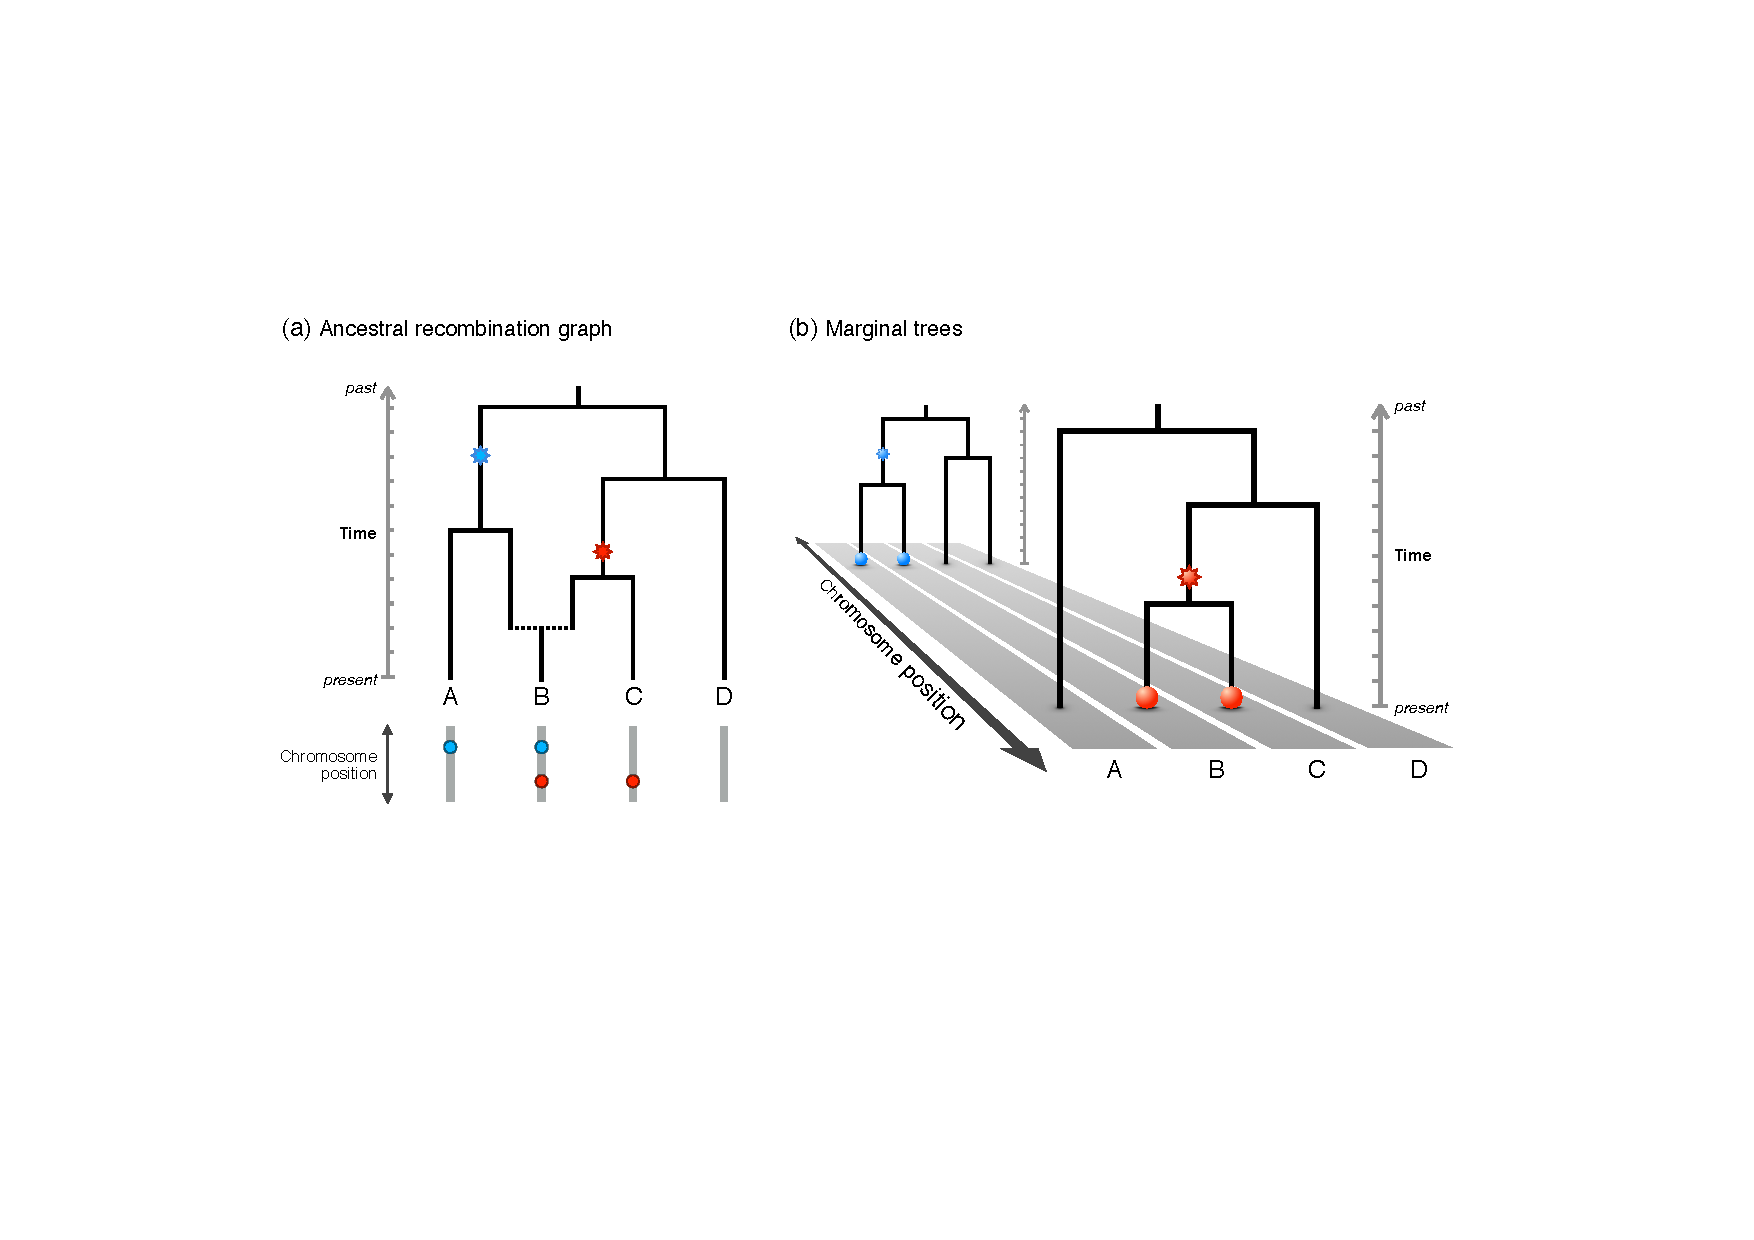
\includegraphics[width=\textwidth]{./img/ch1/info_arg}
\Caption{Illustration of the ancestral recombination graph}
{Panel~\textbf{(a)} shows the \gls{arg} for a sample of \n{4}~chromosomes, labelled by $A$, $B$, $C$, and $D$.
The \emph{dotted} horizontal line denotes the time of a recombination event between chromosomal lineages.
Mutation events are shown as \emph{stars}.
The chromosomal positions of derived alleles are indicated below the \gls{arg}.
The corresponding marginal trees are shown in Panel~\textbf{(b)}, where each lane (\emph{grey}) represents the chromosomal sequence on which the derived alleles sit (shown as \emph{marbles}).}
{fig:info_arg}
% \vspace{-5pt}
% \hrulefill%
\end{figure}
